\documentclass[12pt, twoside]{article}
\usepackage[letterpaper, margin=1in, headsep=0.5in]{geometry}
\usepackage[english]{babel}
\usepackage[utf8]{inputenc}
\usepackage{amsmath}
\usepackage{amsfonts}
\usepackage{amssymb}
\usepackage{tikz}
\usepackage{yhmath}
\usetikzlibrary{quotes, angles}
\usepackage{graphicx}
\usepackage{enumitem}
\usepackage{multicol}

\newif\ifmeta
\metatrue %print standards and topics tags

\title{Regents Geometry}
\author{Chris Huson}
\date{March 2022}

\usepackage{fancyhdr}
\pagestyle{fancy}
\fancyhf{}
\renewcommand{\headrulewidth}{0pt} % disable the underline of the header
\raggedbottom

\fancyhead[LE]{\thepage}
\fancyhead[RO]{\thepage \\ Name: \hspace{4cm} \,\\}
\fancyhead[LO]{BECA / Dr. Huson / Geometry\\* Unit 9: Algebra\\* 21 March 2022}

\begin{document}
\subsubsection*{9.1 Classwork: Algebra skills assessment}
\emph{Do not use a calculator. Do not convert values to decimals.}\\
Reference: Chili Math, Solving Literal Equations \\
https://www.chilimath.com/lessons/intermediate-algebra/literal-equations/

\begin{enumerate}
\subsubsection*{Simplify each expression by ``collecting like terms''}
\item 
\begin{enumerate}[itemsep=2cm]
    \begin{multicols}{2}
      \item $2x+4-x+11$
      \item $5y-4-7y+y$
      \item $14+5\pi-2\pi+4$
      \item $2a+\sqrt{5}+7a+3\sqrt{5}$
      \item $x\sqrt{3}-x\sqrt{3}+x+1$
      \item $3\pi x+4+2 \pi x -7$
    \end{multicols}
    \end{enumerate} \vspace{0.5cm}
  
\subsubsection*{Solve each equation for the unknown}  
One step.
\item 
\begin{enumerate}[itemsep=2cm]
    \begin{multicols}{2}
      \item $2x=12$
      \item $4z=-8$
      \item $3a=\pi$
      \item $2y=\sqrt{5}$
    \end{multicols}
    \end{enumerate} \vspace{1cm}
  
Two steps.
\item 
\begin{enumerate}[itemsep=2cm]
    \begin{multicols}{2}
      \item $7x+4=11$
      \item $-4b+5=-3$
      \item $4m-\sqrt{2}=3\sqrt{2}$
      \item $2y-3\pi=\pi$
    \end{multicols}
    \end{enumerate} 
  
\newpage
\item Fractional coefficients
\begin{enumerate}[itemsep=2cm]
    \begin{multicols}{2}
      \item   $\frac{1}{2}(6-2x)=4x$
      \item   $11=\frac{1}{3}x+2x-10$
    \end{multicols}
    \end{enumerate} \vspace{3cm}

\subsubsection*{Working with polynomials}
\item Simplify each expression by ``collecting like terms''
\begin{enumerate}[itemsep=2cm]
    \begin{multicols}{2}
      \item $4x^2+3x -7 -2x^2-x+4$
      \item $3(a^2-2a +1) -2(a^2-a-4)$
    \end{multicols}
    \end{enumerate} \vspace{2cm}
  
  \subsubsection*{Slope-intercept form}
  \item What is the slope and $y$-intercept of each equation?
\begin{enumerate}[itemsep=2cm]
    \begin{multicols}{2}
      \item   $y=2x-3$
      \item   $4x+2y=6$
    \end{multicols}
    \end{enumerate} \vspace{1.5cm}
  
\subsubsection*{Function substitution}
\item 
\begin{enumerate}[itemsep=2cm]
    \begin{multicols}{2}
      \item Given $f(x)=4x+7$. \\
      Simplify $f(2)$.
      \item Given $\displaystyle f(x)=-\frac{(12+4x)}{11}$. \\
      Simplify $f(-3)$.
    \end{multicols}
    \end{enumerate}


\newpage
\subsubsection*{Parallel and perpendicular linear equations}

  \item What is the equation of the line with a slope of 2 passing through the point $(0,1)$? \\
  hint: $y-y_1=m(x-x_1)$ \vspace{1.5cm}
  \item What is the equation of a line parallel to $y=-2x+1$ with a $y$-intercept of 4? \vspace{1.5cm}
  \item What is the slope of a line perpendicular to the line $x-2y=16$? \vspace{3cm}

\subsubsection*{Rounding and calculations}
  \item Perform each calculation, writing down the full calculator display and then rounding to the \emph{nearest hundredth}.
    \begin{multicols}{2}
    \begin{enumerate}[itemsep=2cm]
      \item $A=15.944732$
      \item $W=3.4 \times 9.8 \times 4.3 \times 0.15$
            
      \item $V=\frac{1}{3} \pi (3.4)^2(6.1)$
      \item $P=8.6 + \frac{1}{2} \pi (8.6)$  
      \item $V=199.19711$
      \item $W=\frac{1}{3} (13)  3.3^2 \times 1.175$
      \item $V=\frac{1}{3} \pi (12.4)^2(8.1)$
      \item $P=12 + \frac{1}{4} \pi (12)$ 
    \end{enumerate}
    \end{multicols}\vspace{2cm}
  
     
  
  \newpage
    \item Oceanside Bike Rental Shop charges a 17 dollar bike fee plus 6 dollars an hour for renting a bike. Jeffrey paid 53 dollars total. How many hours did he pay to have the bike checked out? \vspace{6cm}
  
    \item Three friends go bowling. The cost per person per game is \$5.30. The cost to rent shoes is \$2.50 per person. Their total cost is \$55.20. How many games did they play? \vspace{6cm}
  
    \item The admission fee at a small fair is \$1.50 for children and \$4.00 for adults. On a certain day, 40 people enter the fair and \$85.00 is collected. How many children and how many adults attended?
  
\newpage
\item Solve the system of equations by graphing each line and marking the intersection as an ordered pair.
      \[x+y=7\]
      \[y=3x+3\]
  
  \begin{center} %4 quadrant regents grid
  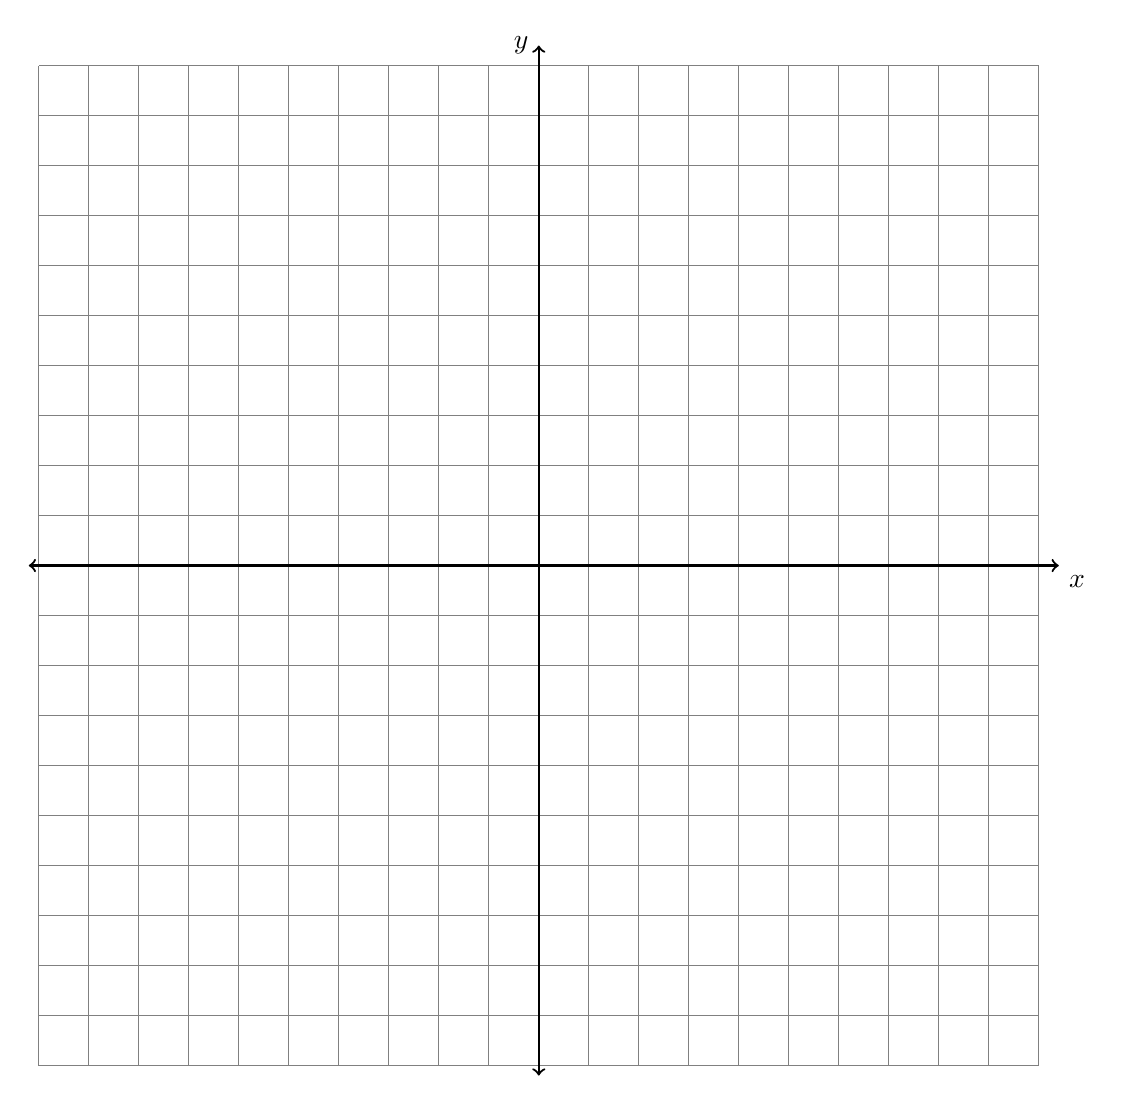
\begin{tikzpicture}[scale=0.635]
    \draw [help lines] (-10,-10) grid (10,10);
    \draw [thick, <->] (-10.2,0) -- (10.4,0) node [below right] {$x$};
    \draw [thick, <->] (0,-10.2)--(0,10.4) node [left] {$y$};
  \end{tikzpicture}
  \end{center}
  
  \newpage
    Solve each system algebraically.
    \item
    $2x-4y=14$\\*
    $5x+4y=7$ \vspace{6cm}
  
    \item
    $2x-y=-7$\\*
    $3x+4y=17$  \vspace{6cm}
      
      

\end{enumerate}
\end{document}
